\begin{definition}[Weighted Type Graph~\cite{endrullis2024generalized_arxiv_v2}]
    \label{wf:def:weighted_type_graph}
    A \textbf{weighted type graph}~\(\mathcal{T} = (T, \mathbb{E}, \mathcal{S}, w)\) consists of:
    \begin{itemize} 
        \item an object \(T\) in $\mathcal{C}$, called \textbf{type graph},
        \item a commutative semiring \(\mathcal{S}=(S, \oplus, \odot, 0_\mathcal{S}, 1_\mathcal{S})\),
        \item a set \(\mathbb{E}\) of morphisms with codomain $T$ in $\mathcal{C}$, called \textbf{morphism-rulers}
        \item a weight function \(w : \mathbb{E} \to S \setminus \{0_\mathcal{S}\}\) such that for all $e \in \mathbb{E}, w(e) \geq 1_\mathcal{S}$.
    \end{itemize}
    \(\mathcal{T}\) is \textbf{finitary} if for every \( (e :X \to T) \in \mathbb{E}\) and every object \(G\), the sets \(\operatorname{Hom}(X, G)\) and \(\operatorname{Hom}(G, T)\) are finite.
\end{definition}

\begin{example}
    \label{wf:example:weighted_type_graph}
     In \textbf{Graph}, a weighted type graph 
     whose $\operatorname{dom}(\mathbb{E})$ consists of graphs with two vertices and one labeled edge between them
     can be visualized as a graph with weighted labels and weights given as superscripts. For example, the finitary weighted type graph $\mathcal{T} = (T, \mathbb{E}, \mathcal{S}, w)$ with $\mathcal{S}$ as the natural arithmetic semiring $(\mathbb{N}, +, *, 0_\mathbb{N}, 1_\mathbb{N}, <,\leq)$,
     $T$ as the graph illustrated below (without superscripts), $\mathbb{E}=\{e_{11a},e_{12a},e_{21a},e_{11b}\}$ as the set of morphism-rulers where 
     $e_{uvl}$ has domain 
     \tikz[baseline=-0.5ex]{
        \node (x) at (0,0) {$\bullet$};
        \node (y) at (1,0) {$\bullet$};
        \draw[->] (x) -- (y) node[midway, above] {$l$};
    } and image 
    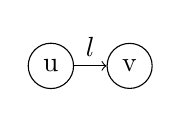
\begin{tikzpicture}
        \node[draw, circle] (x) at (0,0) {$\mathrm{u}$};
        \node[draw, circle] (y) at (1,0) {$\mathrm{v}$};
        \draw[->]  (x) -- (y) node [midway,above] {$l$};
    \end{tikzpicture} in the graph $T$,
    and $w(e) = 1$ for all $e \in \mathbb{E}$, can be visualized as follows:
    \begin{center}
        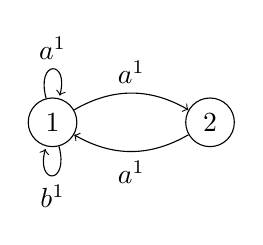
\begin{tikzpicture}
            \graphbox{}{0mm}{0mm}{32mm}{28mm}{-10mm}{-14mm}{
                \node[draw,circle] (1) at (0,0) {1};
                \node[draw,circle] (2) at (2,0) {2};
                \draw[->] (1) edge[loop above] node[midway, above] {$a^{1}$} (1) ;
                \draw[->] (1) edge[loop below] node[midway, below] {$b^{1}$} (1) ;
                \draw[->] (1) edge[bend left] node[midway, above] {$a^{1}$}  (2)  ;
                \draw[->] (2) edge[bend left] node[midway, below] {$a^{1}$} (1)   ;
            }
        \end{tikzpicture}
    \end{center}
\end{example}